
\subsection{Motivation}
Controlled experiments under realistic network conditions is crucial in networking. In this thesis where performance of low-latency applications under time-varying capacity networks like cellular networks, it was important to be able to perform reproducible and realistic experiments on LL applications under cellular networks. To this end, MIT researchers developed a network emulation tool called Mahimahi % reference.
This tool offers the ability to reproduce the behavior of time-varying capacity networks using recorded transmission opportunities (\textit{txops}). However, the txops used by Mahimahi are old and not representative of current cellular network capacities. They were collected on Verizon and TMobile LTE network in 2016 with a downlink throughbout about 5-10 Mbps while the rapport of \ac{ARCEP} \cite{arcepQualitServices} of 2021 report that in France, the downlink throughput on average whatever the location or the network operator used were about 71 Mbps.  Based on this observation, it was important to collect more recent txops file to perform better evaluations.


\subsection{Measurement methodology}
\subsubsection{Mahimahi-LinkShell}
Mahimahi \cite{netravali2015mahimahi} is a framework designed to capture and replay traffic from HTTP-based applications under emulated network conditions. It operates by creating a set of Linux shells, each contained within its own network namespace, meaning that each shell has an isolated network stack with its own routes, firewall, and network devices. Mahimahi includes 04 tools such as LinkShell, RecordShell, DelayShell, and LossShell. Compared to earlier traffic capture and replay tools, Mahimahi offers several advantages: it enables multi-server emulation for web applications and provides network namespace isolation in each shell. This isolation eliminates variability caused by interference from cross-traffic, thus ensuring reproducible experiments. Additionally, Mahimahi's composability and extensibility make it a versatile tool for network research.

\begin{figure*}[!t]
    \centering
    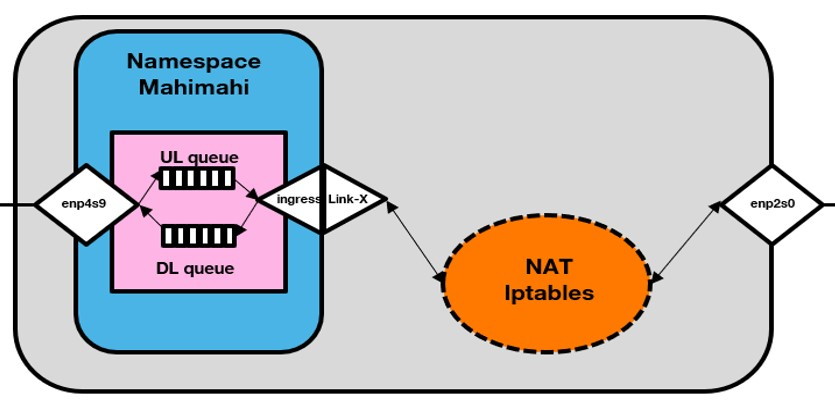
\includegraphics[width=.7\linewidth]{imgs/chapter_2/linkshell.jpg}
    \caption{LinkShell component.}
    \label{fig:chap_2:linkshell}
\end{figure*}

In this thesis, the Mahimahi component of particular interest is LinkShell. LinkShell, depicted in Fig. \ref{fig:chap_2:linkshell}, allows for the emulation of network links, either with a fixed rate or with time-varying conditions, such as those found in cellular networks. To achieve this, LinkShell relies on two transmission opportunity (txops) files: one for uplink and one for downlink network conditions. Each line in a txops file represents a transmission opportunity, defined by a time (in milliseconds) when a \ac{MTU}-sized packet (1500 bytes) can be transferred through the emulated link. Since actual packet sizes can often be smaller than 1500 bytes, a transmission opportunity may allow for the transfer of multiple packets whose combined size equals 1500 bytes. LinkShell queues incoming packets (separately for uplink and downlink) and transmits them during the corresponding transmission opportunity. If no packet is available during a transmission opportunity, that opportunity is wasted.

An example of a txops file is depicted in Fig. \ref{fig:chap_2:txop_file}

\begin{figure*}[!t]
    \centering
    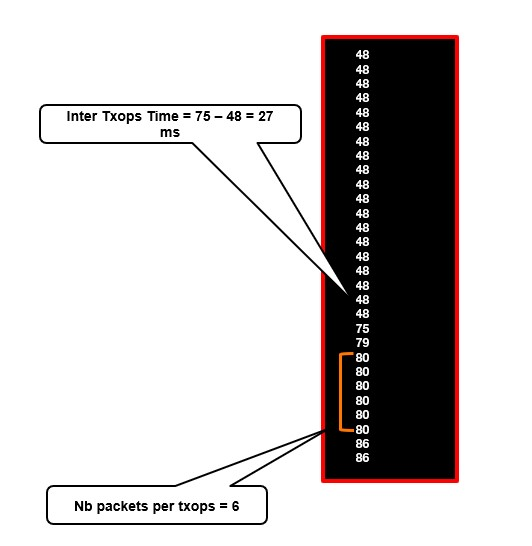
\includegraphics[width=.6\linewidth]{imgs/chapter_2/txops_file.jpg}
    \caption{An example of a txop file.}
    \label{fig:chap_2:txop_file}
\end{figure*}


% Figure with an example of a txops file

\subsubsection{Saturator Tool}
Since the existing txops files are outdated, it was necessary to collect new ones that more accurately reflect the current capacity of cellular networks. For this purpose, we utilized the Saturator tool \footnote{\url{https://github.com/keithw/multisend/blob/master/sender/saturatr.cc}}, which captures network trace samples by saturating the radio link between a User Equipment (UE) and the base station, enabling precise measurement of transmission opportunities. The operation of the Saturator tool is illustrated in Fig. \ref{fig:chap_2:saturator}. 
Our setup consisted of two Xiaomi Mi 10 5G UEs, one Ubuntu 20.04 machine acting as the client, and one Ubuntu 18.04 machine as the server. The client saturated the uplink of the USB-tethered UE, while the server saturated the downlink. Acknowledgements were exchanged between the client and server through a non-saturated WiFi-tethered UE, ensuring accurate communication without interfering with the uplink and downlink saturation. During the process, the client sent timestamped packets to the server, which computed the round-trip time (RTT) upon receiving acknowledgements. The RTT information was then used to adapt the client's congestion window, ensuring continuous saturation of the radio link. A similar process occurred on the server side to keep the radio link between the base station and UE fully saturated.

Once the capture was completed, the raw data collected by the client and server was aggregated and processed to generate two txops files (one for uplink and one for downlink). These files are used by Mahimahi’s LinkShell to emulate time-varying cellular networks, replicating the behavior observed during the experiment.

\begin{figure*}[ht]
    \centering
    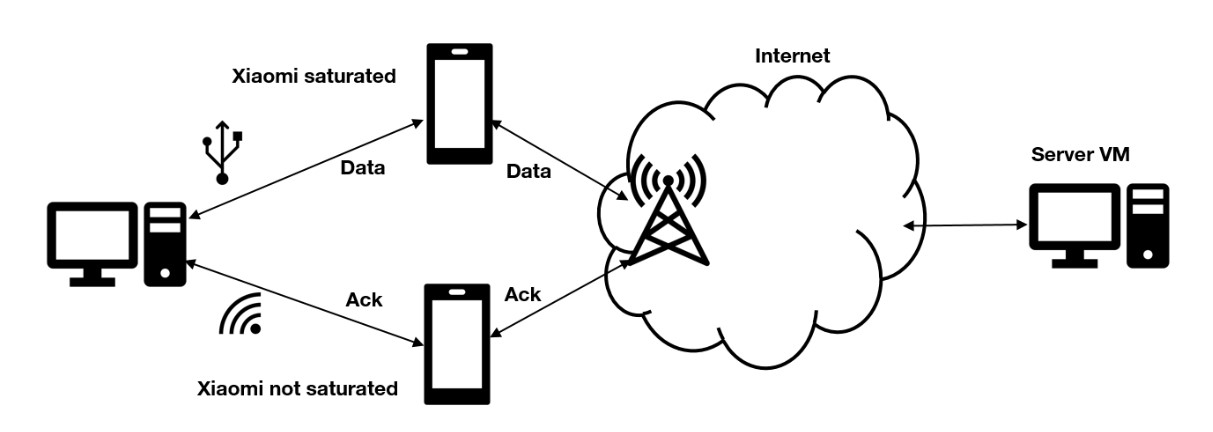
\includegraphics[width=\linewidth]{imgs/chapter_2/saturator.jpg}
    \caption{Saturator tool functioning.}
    \label{fig:chap_2:saturator}
\end{figure*}

\subsubsection{Experiments and results}


\begin{table}[!t]
\begin{threeparttable}
\caption{Characterization of the six txops captured}
\label{tab:chap_2:measurements_conditions}
\setlength\tabcolsep{0pt} % make LaTeX figure out intercolumn spacing

\begin{tabular*}{\columnwidth}{@{\extracolsep{\fill}} l c c c c c c}
\toprule
      \bf Network &  \bf  Mean & \bf Std & \bf \% of time & \bf \% of empty & \bf Location  &  \bf Hour \\
      \bf Conditions &  \bf  (Mbps)  & \bf (Mbps) & \bf $\geq 20$ (Mbps) & \bf period of 33ms & (France) &  \\
\midrule
        \bf Trace E & 230 & 48.7 & 99.9 & 2.6 & Orange Lannion & 2pm \\
\addlinespace
        \bf Trace D & 173.3 & 43.4 & 99.8 & 3.8 & Orange Lannion & 11am \\
\addlinespace
        \bf Trace C & 141.6 & 49.5 & 97.4 & 0.4 & Brélévenez & 9am \\
\addlinespace
        \bf Trace B & 78.8 & 20.3 & 99.5 & 8.0 & Brélévenez & 1pm \\
\addlinespace
        \bf Trace A & 45 & 7.4 & 99.3 & 5.8 & Plemeur-Bodou & 3pm \\
\addlinespace
        \bf Highway & 43.7 & 31.5 & 70.5 & 17.7 & Guingamp - Lannion & 10am \\


\bottomrule
\end{tabular*}
\end{threeparttable}
\end{table}
We conducted txops captures using this setup on the Orange 4G network in January 2022. Each capture lasted for 10 minutes, under varying network conditions, including differences in average bandwidth, bandwidth variability, and time gaps, to ensure the generated txops files would be representative of typical network scenarios. Additionally, we captured txops data during a mobility experiment on a highway between Guingamp and Lannion (France), traveling at 110 km/h. This capture reflected highly variable coverage, with strong signal near urban areas and weak coverage in rural zones.

As a result, six txops files (covering both uplink and downlink) were collected, representing diverse conditions of the Orange 4G network. The experimental conditions and key statistics of the recorded traces are presented in Tab. \ref{tab:chap_2:measurements_conditions}. Further details on the six txops files can be found in the appendix \ref{txops_annex}. % Add reference and figure



\takeaway{We collect in this experiment new txops files that will be used in the rest of our work for data collection on CG platforms but could also serve for other use-cases like performance evaluation of web applications under cellular network conditions \cite{mathieu2021evaluating} or for congestion control evaluation.

As such, the datasets are available as OpenData : \url{https://cloud-gaming-traces.lhs.inria.fr/ANR-19-CE25-0012_Mahimahi_Orange_4G_traces_January_2022.zip}}
